% Options for packages loaded elsewhere
\PassOptionsToPackage{unicode}{hyperref}
\PassOptionsToPackage{hyphens}{url}
%
\documentclass[
]{article}
\usepackage{lmodern}
\usepackage{amssymb,amsmath}
\usepackage{ifxetex,ifluatex}
\ifnum 0\ifxetex 1\fi\ifluatex 1\fi=0 % if pdftex
  \usepackage[T1]{fontenc}
  \usepackage[utf8]{inputenc}
  \usepackage{textcomp} % provide euro and other symbols
\else % if luatex or xetex
  \usepackage{unicode-math}
  \defaultfontfeatures{Scale=MatchLowercase}
  \defaultfontfeatures[\rmfamily]{Ligatures=TeX,Scale=1}
\fi
% Use upquote if available, for straight quotes in verbatim environments
\IfFileExists{upquote.sty}{\usepackage{upquote}}{}
\IfFileExists{microtype.sty}{% use microtype if available
  \usepackage[]{microtype}
  \UseMicrotypeSet[protrusion]{basicmath} % disable protrusion for tt fonts
}{}
\makeatletter
\@ifundefined{KOMAClassName}{% if non-KOMA class
  \IfFileExists{parskip.sty}{%
    \usepackage{parskip}
  }{% else
    \setlength{\parindent}{0pt}
    \setlength{\parskip}{6pt plus 2pt minus 1pt}}
}{% if KOMA class
  \KOMAoptions{parskip=half}}
\makeatother
\usepackage{xcolor}
\IfFileExists{xurl.sty}{\usepackage{xurl}}{} % add URL line breaks if available
\IfFileExists{bookmark.sty}{\usepackage{bookmark}}{\usepackage{hyperref}}
\hypersetup{
  pdftitle={linear norm plot},
  pdfauthor={Joshua},
  hidelinks,
  pdfcreator={LaTeX via pandoc}}
\urlstyle{same} % disable monospaced font for URLs
\usepackage[margin=1in]{geometry}
\usepackage{graphicx,grffile}
\makeatletter
\def\maxwidth{\ifdim\Gin@nat@width>\linewidth\linewidth\else\Gin@nat@width\fi}
\def\maxheight{\ifdim\Gin@nat@height>\textheight\textheight\else\Gin@nat@height\fi}
\makeatother
% Scale images if necessary, so that they will not overflow the page
% margins by default, and it is still possible to overwrite the defaults
% using explicit options in \includegraphics[width, height, ...]{}
\setkeys{Gin}{width=\maxwidth,height=\maxheight,keepaspectratio}
% Set default figure placement to htbp
\makeatletter
\def\fps@figure{htbp}
\makeatother
\setlength{\emergencystretch}{3em} % prevent overfull lines
\providecommand{\tightlist}{%
  \setlength{\itemsep}{0pt}\setlength{\parskip}{0pt}}
\setcounter{secnumdepth}{-\maxdimen} % remove section numbering
\usepackage{booktabs}
\usepackage{longtable}
\usepackage{array}
\usepackage{multirow}
\usepackage{wrapfig}
\usepackage{float}
\usepackage{colortbl}
\usepackage{pdflscape}
\usepackage{tabu}
\usepackage{threeparttable}
\usepackage{threeparttablex}
\usepackage[normalem]{ulem}
\usepackage{makecell}
\usepackage{xcolor}

\title{linear norm plot}
\author{Joshua}
\date{15/05/2020}

\begin{document}
\maketitle

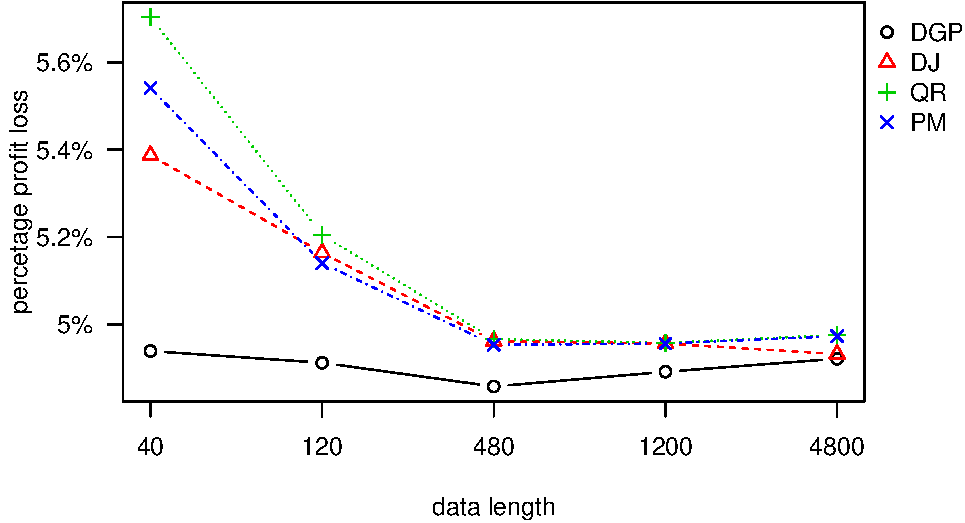
\includegraphics{linear-norm-plot_files/figure-latex/ppl0.5-1.pdf}

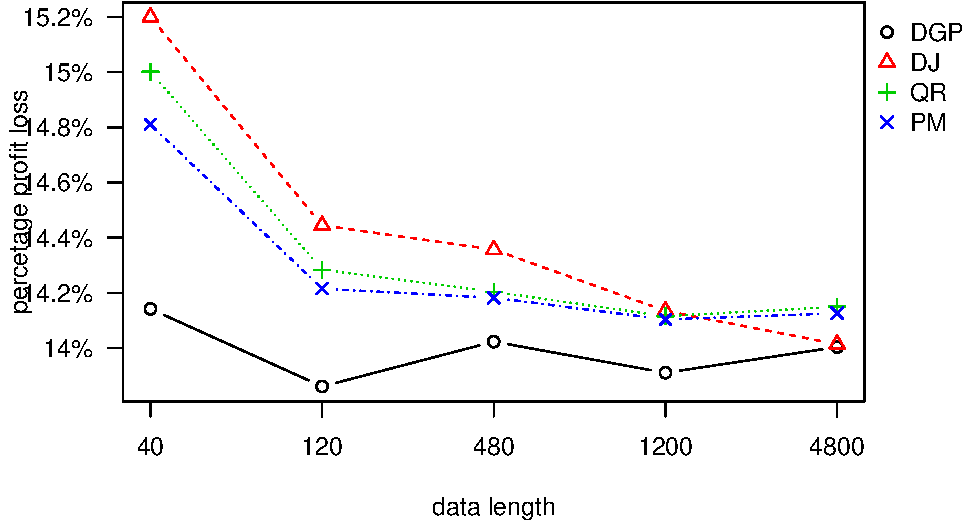
\includegraphics{linear-norm-plot_files/figure-latex/ppl0.63-1.pdf}

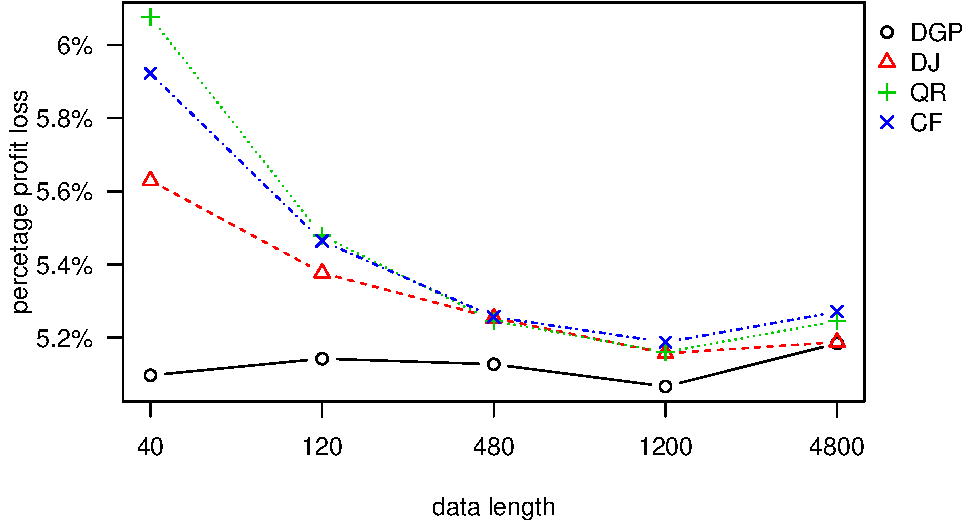
\includegraphics{linear-norm-plot_files/figure-latex/ppl0.3-1.pdf}

\begin{table}

\caption{\label{tab:inventory_error}Inventory Error}
\centering
\resizebox{\linewidth}{!}{
\begin{tabular}[t]{ccccccccccccc}
\toprule
\multicolumn{1}{c}{\textbf{ }} & \multicolumn{4}{c}{\textbf{Target service level=0.5}} & \multicolumn{4}{c}{\textbf{Target service level=0.63}} & \multicolumn{4}{c}{\textbf{Target service level=0.3}} \\
\cmidrule(l{3pt}r{3pt}){2-5} \cmidrule(l{3pt}r{3pt}){6-9} \cmidrule(l{3pt}r{3pt}){10-13}
Data size & DGP & disjoint & quantile & proposed & DGP & disjoint & quantile & proposed & DGP & disjoint & quantile & proposed\\
\midrule
\rowcolor{gray!6}  40 & 0.7 & 32.98 & -0.48 & -0.16 & -89.49 & -47.68 & -60.64 & -62.2 & 135.99 & 151.12 & 106.49 & 96.5\\
 & (200.12) & (220.85) & (232.6) & (225.62) & (200.93) & (222.85) & (234.95) & (227.4) & (199.9) & (222.22) & (236.44) & (227.4)\\
\rowcolor{gray!6}  120 & 2.01 & 14.07 & 1.96 & 1.96 & -74 & -60.69 & -69.19 & -65.85 & 114.32 & 125.76 & 106.21 & 101.36\\
 & (200.57) & (211.5) & (211.92) & (209.86) & (200.59) & (211.19) & (211.79) & (209.24) & (200.74) & (211.37) & (212.14) & (210.26)\\
\rowcolor{gray!6}  480 & 1.16 & 4.12 & 0.88 & 0.97 & -70.42 & -67.98 & -70.15 & -68.47 & 107.98 & 111.99 & 107.12 & 104.83\\
\addlinespace
 & (201.43) & (206.98) & (205.86) & (205.4) & (198.37) & (204.57) & (202.44) & (202.05) & (199.73) & (205.23) & (203.95) & (203.64)\\
\rowcolor{gray!6}  1200 & -0.51 & 1.17 & -0.35 & -0.34 & -66.07 & -66.12 & -66.47 & -65.29 & 105.68 & 109.2 & 106.36 & 104.39\\
 & (200.63) & (204.61) & (203.62) & (203.35) & (197.66) & (201.9) & (200.7) & (200.68) & (197.75) & (202.4) & (201.04) & (201.18)\\
\rowcolor{gray!6}  4800 & 2.88 & 3.45 & 3.19 & 3.12 & -67.63 & -67.33 & -68.16 & -66.98 & 106.33 & 107.18 & 106.99 & 105.37\\
 & (201.31) & (201.67) & (203.23) & (203.19) & (201.55) & (201.96) & (204.19) & (204.21) & (200.96) & (201.37) & (203.04) & (203.37)\\
\bottomrule
\end{tabular}}
\end{table}

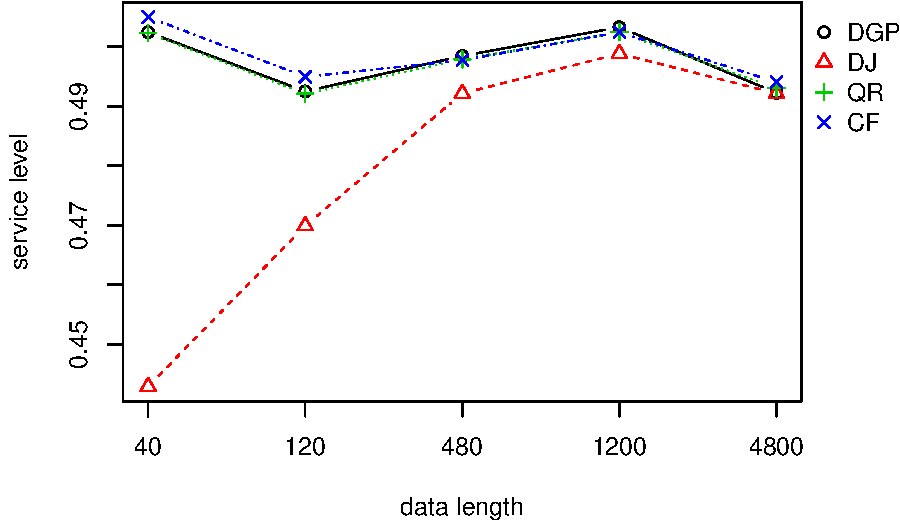
\includegraphics{linear-norm-plot_files/figure-latex/sl-1.pdf}
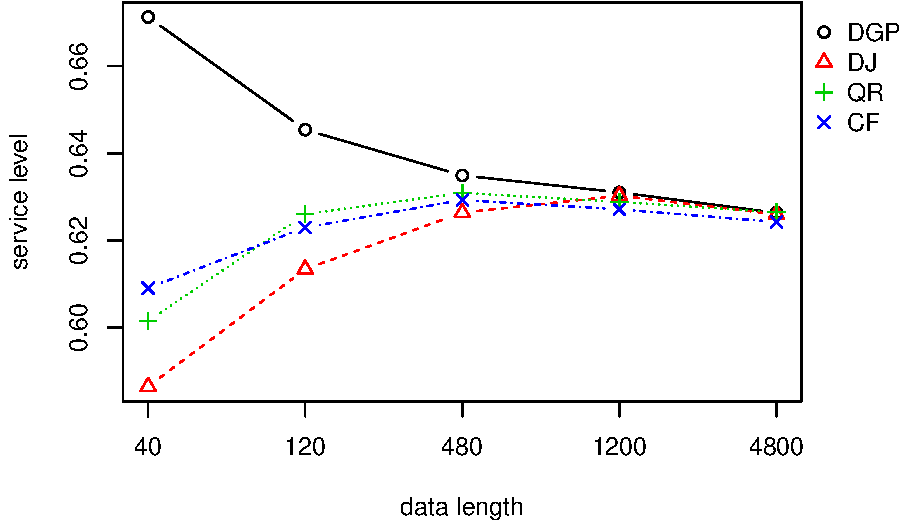
\includegraphics{linear-norm-plot_files/figure-latex/sl-2.pdf}
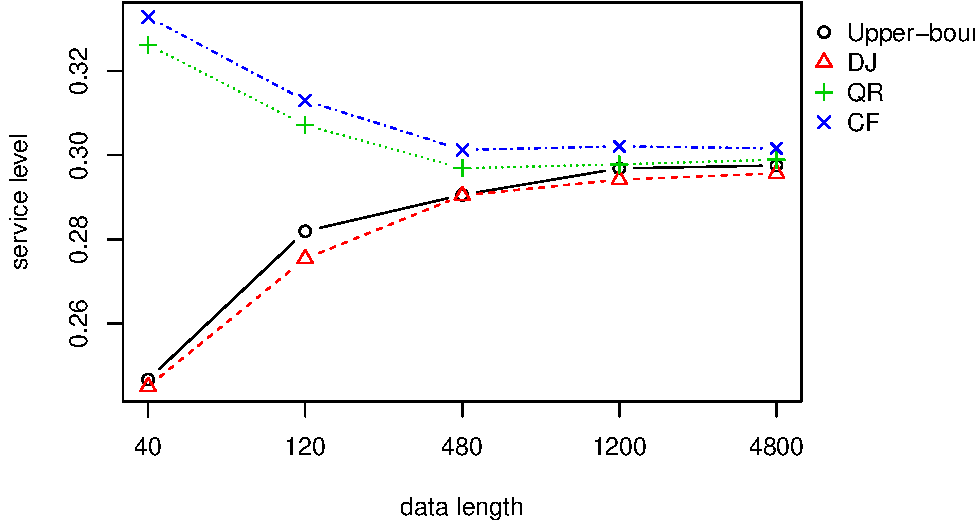
\includegraphics{linear-norm-plot_files/figure-latex/sl-3.pdf}

\begin{table}

\caption{\label{tab:Wilcoxon}p-value of Wilcoxon Test between data size 1200 and 4800}
\centering
\begin{tabular}[t]{ccccc}
\toprule
Target service level & DGP & disjoint & quantile & proposed\\
\midrule
\rowcolor{gray!6}  0.5 & 0.0271056 & 0.1802333 & 0.0601088 & 0.0929595\\
0.63 & 0.3306834 & 0.3736361 & 0.6268995 & 0.5490250\\
\rowcolor{gray!6}  0.3 & 0.8782706 & 0.7505065 & 0.8015530 & 0.9132690\\
\bottomrule
\end{tabular}
\end{table}

\begin{verbatim}
##            DGP        DJ        QR        CF
## 40   0.9515126 0.9332624 0.9427216 0.9444745
## 120  0.9510048 0.9432327 0.9480915 0.9486686
## 480  0.9512050 0.9482805 0.9502174 0.9503142
## 1200 0.9520155 0.9501517 0.9513423 0.9513992
## 4800 0.9507583 0.9503720 0.9503585 0.9503930
\end{verbatim}

\begin{verbatim}
##            DGP        DJ        QR        CF
## 40   0.9746412 0.9586198 0.9594740 0.9617508
## 120  0.9716568 0.9654879 0.9679448 0.9675858
## 480  0.9712849 0.9689282 0.9702442 0.9698065
## 1200 0.9705059 0.9693490 0.9699419 0.9695206
## 4800 0.9699385 0.9697061 0.9694787 0.9690286
\end{verbatim}

\begin{verbatim}
##            DGP        DJ        QR        CF
## 40   0.8953463 0.8804924 0.9003852 0.9075537
## 120  0.9061819 0.8968225 0.9071205 0.9103971
## 480  0.9091751 0.9051790 0.9086960 0.9104068
## 1200 0.9105881 0.9074906 0.9096523 0.9110585
## 4800 0.9096004 0.9090085 0.9089646 0.9101982
\end{verbatim}

\textbackslash begin\{table\}

\textbackslash caption\{\label{tab:size0.5}Size effect (q=50\%)\}
\centering \resizebox{\linewidth}{!}{
\begin{tabular}[t]{ccccccccc}
\toprule
\multicolumn{1}{c}{\textbf{ }} & \multicolumn{4}{c}{\textbf{Percentage profit loss}} & \multicolumn{4}{c}{\textbf{Average service level}} \\
\cmidrule(l{3pt}r{3pt}){2-5} \cmidrule(l{3pt}r{3pt}){6-9}
Data size & DGP & disjoint & quantile & proposed & DGP & disjoint & quantile & proposed\\
\midrule
40 & 4.91\% & 5.35\% & 5.67\% & 5.51\% & 0.502 & 0.443 & 0.502 & 0.505\\
120 & 4.94\% & 5.15\% & 5.20\% & 5.15\% & 0.492 & 0.470 & 0.492 & 0.495\\
480 & 4.94\% & 5.05\% & 5.05\% & 5.04\% & 0.498 & 0.492 & 0.498 & 0.498\\
1200 & 4.92\% & 5.00\% & 4.99\% & 4.99\% & 0.503 & 0.499 & 0.502 & 0.502\\
4800 & 4.92\% & 4.92\% & 4.96\% & 4.96\% & 0.492 & 0.492 & 0.493 & 0.494\\
\bottomrule
\end{tabular}} \textbackslash end\{table\}

\begin{table}

\caption{\label{tab:level40}Target service level effect (n=40)}
\centering
\resizebox{\linewidth}{!}{
\begin{tabular}[t]{ccccccccc}
\toprule
\multicolumn{1}{c}{\textbf{ }} & \multicolumn{4}{c}{\textbf{Percentage profit loss}} & \multicolumn{4}{c}{\textbf{Average service level}} \\
\cmidrule(l{3pt}r{3pt}){2-5} \cmidrule(l{3pt}r{3pt}){6-9}
Target service level & DGP & disjoint & quantile & proposed & DGP & disjoint & quantile & proposed\\
\midrule
\rowcolor{gray!6}  0.5 & 4.91\% & 5.35\% & 5.67\% & 5.51\% & 0.502 & 0.443 & 0.502 & 0.505\\
0.63 & 14.28\% & 15.25\% & 16.15\% & 15.62\% & 0.671 & 0.586 & 0.601 & 0.609\\
\rowcolor{gray!6}  0.3 & 5.10\% & 5.63\% & 6.08\% & 5.92\% & 0.247 & 0.245 & 0.326 & 0.333\\
\bottomrule
\end{tabular}}
\end{table}

\begin{table}

\caption{\label{tab:level480}Target service level effect (n=480)}
\centering
\resizebox{\linewidth}{!}{
\begin{tabular}[t]{ccccccccc}
\toprule
\multicolumn{1}{c}{\textbf{ }} & \multicolumn{4}{c}{\textbf{Percentage profit loss}} & \multicolumn{4}{c}{\textbf{Average service level}} \\
\cmidrule(l{3pt}r{3pt}){2-5} \cmidrule(l{3pt}r{3pt}){6-9}
Target service level & DGP & disjoint & quantile & proposed & DGP & disjoint & quantile & proposed\\
\midrule
\rowcolor{gray!6}  0.5 & 4.94\% & 5.05\% & 5.05\% & 5.04\% & 0.498 & 0.492 & 0.498 & 0.498\\
0.63 & 13.82\% & 14.15\% & 14.10\% & 14.04\% & 0.635 & 0.626 & 0.631 & 0.629\\
\rowcolor{gray!6}  0.3 & 5.13\% & 5.25\% & 5.25\% & 5.26\% & 0.291 & 0.290 & 0.297 & 0.301\\
\bottomrule
\end{tabular}}
\end{table}

\begin{table}

\caption{\label{tab:level4800}Target service level effect (n=4800)}
\centering
\resizebox{\linewidth}{!}{
\begin{tabular}[t]{ccccccccc}
\toprule
\multicolumn{1}{c}{\textbf{ }} & \multicolumn{4}{c}{\textbf{Percentage profit loss}} & \multicolumn{4}{c}{\textbf{Average service level}} \\
\cmidrule(l{3pt}r{3pt}){2-5} \cmidrule(l{3pt}r{3pt}){6-9}
Target service level & DGP & disjoint & quantile & proposed & DGP & disjoint & quantile & proposed\\
\midrule
\rowcolor{gray!6}  0.5 & 4.92\% & 4.92\% & 4.96\% & 4.96\% & 0.492 & 0.492 & 0.493 & 0.494\\
0.63 & 14.02\% & 14.04\% & 14.22\% & 14.20\% & 0.626 & 0.626 & 0.626 & 0.624\\
\rowcolor{gray!6}  0.3 & 5.18\% & 5.19\% & 5.25\% & 5.27\% & 0.298 & 0.296 & 0.299 & 0.302\\
\bottomrule
\end{tabular}}
\end{table}

\end{document}
